\documentclass[12pt]{article}
\usepackage[paper=letterpaper,margin=1.5cm]{geometry}
\usepackage{amsmath}
\usepackage{amssymb}
\usepackage{amsfonts}
\usepackage{mathtools}
\usepackage[utf8]{inputenc}
\usepackage{newtxtext, newtxmath}
\usepackage{enumitem}
\usepackage{titling}
\usepackage{graphicx}
\usepackage[colorlinks=true]{hyperref}
\usepackage{setspace}
\usepackage{braket}
\usepackage{color}

\setlength{\droptitle}{-6em}

\newcommand{\hop}{\vspace{1mm}}
\newcommand{\jump}{\vspace{5mm}}
\newcommand{\R}{\mathbb{R}}
\newcommand{\C}{\mathbb{C}}
\newcommand{\bt}{\textbf}
\newcommand{\lm}{\lambda}
\newcommand{\ep}{\varepsilon}
\definecolor{cit}{rgb}{0.05,0.2,0.45}
\addtolength{\jot}{1em}
\newcommand{\solution}[1]{

\vspace{5mm}
\medskip\noindent{\color{cit}\textbf{Solution:} #1}}

% Enter the specific assignment number and topic of that assignment below, and replace "Your Name" with your actual name.
\title{STAT 31410: Homework 1}
\author{Caleb Derrickson}
\date{October 8, 2023}

\begin{document}
\onehalfspacing
\maketitle

For this problem set, we consider the equation for an idealized pendulum
\begin{align}
    \frac{d^2\theta}{dt^2} = -\frac{g}{\ell(t)}sin(\theta), \label{Original ode}
\end{align}

where the length of the moment arm, $l$, varies periodically according to

\begin{align}
    \ell (t) = \ell_0(1 + \ep \cos(\omega t)), \hspace{5mm} \ep \ll 1.    \label{length approx}
\end{align}

This might be a good model of a child on a swing, trying to pump energy into it by repeatedly
standing up and then squatting back down with some appropriate rhythm, to be determined.

\jump
\centerline{\noindent}%
\makebox[\textwidth]{
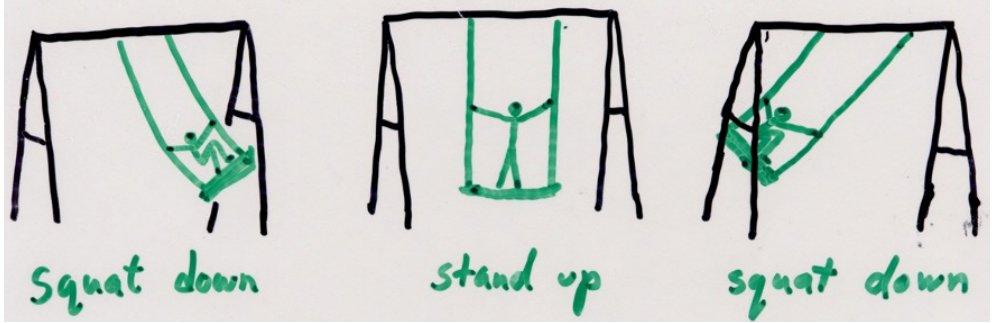
\includegraphics[scale = 0.6]{Images/swing.PNG}
}
\jump

\begin{enumerate}
    \item Make an approximation where you keep only the leading order term in $\ep$, i.e linearize about $\varepsilon$ = 0. Then choose a non-dimensionalization of time that puts (1) into this form:

    \begin{align}
        \ddot{\theta} = -(\alpha + \beta \cos(\tau))\sin(\theta),   \label{linearish}
    \end{align}

        where you define the dimensionless parameters $\alpha$ and $\beta$ in terms of the original parameters $g$, $\ell_0$, $\varepsilon$ and $\omega$. Re-write the second order equation \ref{linearish} as two first order equations for the angle $\theta$ and the angular speed $\omega \equiv \dot{\theta}$. For $\beta$ = 0, derive a conserved quantity, the energy of the pendulum, denoted $E(\theta, \Omega)$. Write an equation for $\dot{E}$ that applies if $\beta \neq 0$.

        {\color{cit}\vspace{2mm}\noindent\textbf{Collaborators:}} The TA's of the class, as well as Kevin Hefner, Nathan Suhr, and Steven Lee.
        \begin{solution}

        Since we are taking $\ep \ll 1$ from \ref{Original ode}, we can define a function $f(\ep)$ on which we will expand using ordinary Taylor expansion. Here, I will define $f(\ep)$ as:
        \begin{align}
            f(\ep) = \frac{1}{1 + \ep \cos(\omega t)},
        \end{align}

        where it is understood that $\cos(\omega t)$ is a constant in this sense. Note that we are \textit{linearizing} with respect to $\theta$, so we can drop all terms of higher order. Thus, 

        \begin{align}
            f(\ep) &= \sum_{n = 0}^\infty \ep^n\frac{d^nf}{d\ep^n} \Big\rvert_{\ep = 0} \nonumber \\
            &= f(\ep = 0) + \ep\frac{df}{d\ep} \Big\rvert_{\ep = 0} + O(n^2)  \nonumber \\
            &= 1 - \ep \bigg[ \frac{\cos(\omega t)}{(1 + \ep\cos(\omega t))^2} \bigg]_{\ep = 0}  \nonumber \\
            & = 1 - \ep \cos(\omega t) \label{Expansion} 
        \end{align}

        We can then plug \ref{Expansion} into \ref{Original ode} to obtain,

        \begin{align}
            \ddot{\theta} = -\frac{g}{\ell_0}\Big(1 - \ep \cos(\omega t)\Big)\sin(\theta). \label{before parameters}
        \end{align}

        From \ref{before parameters}, we can define three dimensionless parameters: $\tau, \alpha, \beta$. $\tau$ will take the place of the argument inside the cosine term of \ref{before parameters}, while $\alpha$ and $\beta$ will clean up any extraneous terms. We will first redefine the ratio of $g$ and $\ell_0$ as the resonance frequency of our state, $\omega_0$.
        
        \begin{align*}
            \omega_0^2 = \frac{\ell_0}{g}.    
        \end{align*}

        Then we will take $\tau$ as $\tau = \omega t$. Note that we are taking time derivatives, so this re-parameterization affects what we are differentiating by. 

        \begin{align*}
            \tau = \omega t \implies d\tau = \omega dt \iff \frac{1}{\omega}\frac{d}{d\tau} = \frac{d}{dt}.
        \end{align*}

        Applying these to \ref{before parameters}, we get,

        \begin{align}
            \ddot{\theta} = -\Big(\frac{\omega_0}{\omega} \Big)^2 \big( 1 - \ep \cos(\tau) \big) \sin(\theta).  \label{before alphabeta}
        \end{align}

        We can then define $\alpha, \beta$ as,

        \begin{align}
            \alpha = \bigg(\frac{\omega_0}{\omega}\bigg)^2, \hspace{10mm} \beta = \alpha\ep
        \end{align}

        Note that, as suggested by the TA's, to take $\beta$ as a positive constant. The negative can be recovered by shifting $\tau$ by $\pi$, meaning $\tau = \omega t + \pi$. This shift will change nothing else in our analysis, hopefully. Also, when taking time derivates for the rest of this homework, I am specifically referring to taking the $\tau$ derivative. Thus, our second order differential equation is, 

        \begin{align}
            \ddot{\theta} = -\big(\alpha + \beta \cos(\tau)\big)\sin(\theta),   \label{second order ode with new parameters}
        \end{align}

        matching \ref{linearish}. 

        Our next goal is to re-write \ref{second order ode with new parameters} as two first order equations for $\theta$ and the angular speed $\Omega \equiv \dot{\theta}$. This can be achieved quite easily - our system is now. 
        \begin{equation}
        \begin{cases}
            \dot{\theta} = \Omega, \\
            \dot{\Omega} = -\big(\alpha + \beta \cos(\tau)\big)\sin(\theta)
        \end{cases}    
        \end{equation}

        Our next goal is to find a conserved quantity for $\beta = 0$. This quantity will be the energy of our system (or rather, an approximation of it) and will be denoted as $E$. From the lectures, our energy is the sum of kinetic and potential energies, in just the $\theta$ dimension. Potential can be found by integrating the (negative) right-hand-side of \ref{second order ode with new parameters} by our spacial parameter. 

        \begin{align}
            \implies V(\theta) &= \int \alpha\sin(\theta) \ d\theta \nonumber\\
            &= -\big(\alpha + \beta\cos(\tau))\cos(\theta)
        \end{align}

        The energy is now,

        \begin{align}
            E(\theta, \Omega) &= \frac{1}{2} \dot{\theta}^2 + V(\theta),    \nonumber   \\
            &= \frac{1}{2} \Omega^2 -\alpha\cos(\theta).
        \end{align}

        Where the instantaneous change in energy (with respect to time) is,

        \begin{align}
            \dot{E}(\theta, \Omega) &=  \frac{d}{d\tau}\bigg[ \frac{1}{2}\Omega^2 - \alpha\cos(\theta) \bigg]  \nonumber\\
            &= \Omega\dot{\Omega} - \alpha\frac{d}{d\tau}\bigg[ \cos(\theta) \bigg] \nonumber\\
            &= -\Omega\big(\alpha + \beta \cos(\tau)\big)\sin(\theta) + \alpha\sin(\theta)\dot{\theta}\nonumber\\
            &= -\beta\Omega\cos(\tau)\sin(\theta)
        \end{align}
        \end{solution}
\end{enumerate}
\end{document}